% !TEX program = pdflatex
\documentclass[11pt,a4paper]{article}

\usepackage[english]{babel}
\usepackage[margin=2.5cm]{geometry}
\usepackage{setspace}
\onehalfspacing

\usepackage{amsmath,amssymb,amsthm}
\usepackage{mathtools}
\usepackage{bm}

\newtheorem{theorem}{Theorem}[section]
\newtheorem{lemma}[theorem]{Lemma}
\newtheorem{proposition}[theorem]{Proposition}
\newtheorem{corollary}[theorem]{Corollary}
\newtheorem{definition}[theorem]{Definition}
\newtheorem{remark}[theorem]{Remark}
\theoremstyle{definition}
\newtheorem{condition}[theorem]{Condition}

\usepackage{graphicx}
\usepackage{float}
\usepackage{booktabs}
\usepackage{multirow}
\usepackage{array}
\usepackage{caption}
\usepackage{subcaption}

\usepackage[colorlinks=true,linkcolor=blue,citecolor=blue,urlcolor=blue]{hyperref}

\usepackage{csquotes}
\usepackage[style=authoryear-comp,backend=biber]{biblatex}
\addbibresource{references.bib}

\usepackage{enumitem}
\usepackage{tikz}
\usetikzlibrary{arrows.meta,positioning,shapes,fit,backgrounds}
\usepackage{mdframed}
\usepackage{xcolor}

\definecolor{lightgray}{RGB}{245,245,245}
\definecolor{lightblue}{RGB}{230,240,250}
\definecolor{lightred}{RGB}{255,240,240}

\newcommand{\verifspace}{\mathcal{C}_{\mathcal{V}}}
\newcommand{\taskcspace}{\mathcal{C}}
\newcommand{\effcap}{\mathcal{E}}
\newcommand{\contextcap}{\mathcal{W}}

\title{{\bfseries Convergence and Divergence:\\Capability Boundaries, Structural Deficiencies,\\and the Necessity of Human-AI Collaboration in LLM Agents}}

\author{}

\date{\today}

\begin{document}
\maketitle

\begin{abstract}
\noindent
Contemporary LLM-based agent systems exhibit a stable set of failure modes in engineering practice---semantic drift in multi-step planning, the unreliability of fully autonomous closed-loop operation, and structural degradation of cross-session memory. These patterns diminish with each generation of model improvement yet persist without being eliminated. Mainstream research tends to attribute these failures to engineering-level inadequacies such as noise accumulation, context overload, or planning-execution decoupling, and appeals to larger models, longer context windows, or more refined prompt engineering for remediation. This paper advances a fundamentally different thesis: a substantial fraction of these failures are not engineering problems awaiting solution, but structural necessities derivable from the mathematical structure of the current Transformer architecture.

The argument proceeds as follows. First, grounded in the conditional probability mapping property of softmax attention and the finite-dimensional truncation of parameter space, we establish a dual-mode classification framework of training convergence and test convergence. Second, we demonstrate that no continuous transitional structure exists between long-term and short-term memory---parameterized long-term memory and contextual short-term memory belong to different mathematical categories, a fact unaltered by engineering extensions of the context window. Building on this foundation, we partition agent behavior by evaluation mode into convergent tasks (those possessing automatically executable verification criteria) and divergent tasks (those for which verification criteria are absent or non-formalizable). For convergent tasks, we develop a theory of test convergence and prove, in syllogistic form, the structural unreliability of context-driven task decomposition, deriving the closure constraint that root requirements must be externally anchored. For divergent tasks, we reduce the notion of ``exploration'' to a mechanism of conditional probability sampling and construct a theory of preference-driven iteration, demonstrating that in the absence of verification signals, human comparative judgment constitutes the sole directional gradient. Finally, proceeding from three structural deficiencies of agents relative to humans, we systematically derive the irreplaceable role of the human operator in human-AI collaboration and delineate the feasible design space under current mathematical constraints.

The primary contributions of this paper are: (1) a dual-mode classification of training convergence and test convergence that unifies agent behavior under a single convergence-constraint framework; (2) a proof, from the structural difference of the two memory types, that no intermediate transitional memory structure exists between the long and the short term; (3) a syllogistic demonstration that the unreliability of context-driven decomposition decisions is not an empirical contingency but a structural necessity; (4) a theory of preference-driven iteration for divergent tasks, forming a dual to the theory of convergent tasks; and (5) a systematic derivation, from the structural deficiencies of agents, of the constitutive role of the human operator in human-AI collaboration, together with an explicit delineation of the feasible design space.

The paper employs a six-tier hierarchy of argument strength---rigorous tier, definitional tier, formal-demonstrative tier, conceptual-constructive tier, analogical tier, and empirical-inferential tier---with the tier of each section explicitly labeled in the text. No conceptual construction is presented under the guise of a mathematical theorem.
\end{abstract}

\newpage
\tableofcontents
\newpage

% ===================================================================
\section{Introduction: From Usage Principles to Theoretical Motivation}
\label{sec:intro}
% ===================================================================

\subsection{Seventeen Usage Principles: Empirical Induction}

The following principles emerge from systematic observation and induction of LLM agent behavior in the author's long-term engineering practice. Each principle has been repeatedly validated in use, yet the unified mechanism underlying their effectiveness has not been adequately explained by existing theory. This section presents these principles as propositions, serving as the empirical starting point for the theoretical construction that follows. Each principle is assigned a label (P1--P17) for ease of cross-reference in subsequent sections.

\medskip
\textbf{Group I: Input Principles (P1--P3)}

\textbf{P1 (Precision over brevity):} Clarity of informational role in the prompt takes priority over minimizing text length. A finite-dimensional, precise input reduces the structural complexity of the information, raising the probability that the input falls within the region of convergence coverage.

\textbf{P2 (The distributional field effect of words):} The efficacy of a word within a model does not originate from its lexical semantic definition, but from the pragmatic contexts in which it typically appears in the training data. To induce criticality, using words such as ``critique'' or ``matter-of-fact''---which routinely appear in contexts demanding rigor---is more effective than directly employing the abstract label ``objective.'' This phenomenon is a direct manifestation of the principle of distributional semantics: the semantic identity of a linguistic unit is uniquely determined by the totality of conditional probability relations directed toward it from all other units.

\textbf{P3 (Constrain the goal, not the path):} Specify the objective, boundary conditions, and verification criteria to the model; do not prescribe specific implementation steps. Every additional path-level instruction introduces an additional dimension of potential semantic ambiguity, which amplifies, exponentially in the conditional probability space, the probability of drifting outside the region of convergence coverage.

\medskip
\textbf{Group II: Context Management Principles (P4--P5)}

\textbf{P4 (Judicious selection of contextual information):} Every piece of information injected into the context window must be evaluated for its information-theoretic value. The effective context capacity of a model is markedly smaller than the nominal window length; the attention mechanism structurally imposes equal-weight coverage over all information within the window, with redundant information and critical information competing without priority differentiation for limited representational resources in the attention computation.

\textbf{P5 (Tiered, rolling management of context):} Context content is organized hierarchically by information priority. High-priority information (task objectives, constraints, verified intermediate results) is retained persistently within the window; low-priority information is rolled out along a priority gradient as the window advances. This strategy constitutes the information-theoretically optimal allocation under the constraint of finite effective capacity.

\medskip
\textbf{Group III: Convergent Task Principles (P6--P10)}

\textbf{P6 (Node partitioning at the capability boundary):} Task decomposition is performed at the effective boundary of the model's textual input. Information exceeding this boundary is not covered by training convergence constraints; only by partitioning it back within the boundary can the forging effect of convergence constraints on mapping behavior be restored, thereby creating operational space for test convergence.

\textbf{P7 (Test convergence as the driver):} Agent behavior at runtime is driven not by gradient descent but by an iterative cycle of ``generate--verify--analyze--revise.'' Parameters are statically frozen after training; the channel of training convergence is closed. Agent behavior can only be guided by test convergence, which is in turn driven by verifiable objectives.

\textbf{P8 (External constraint anchoring):} Critical branching decisions in task decomposition must be arbitrated by hard constraints independent of the model---either human-defined rules or program logic---and must not be left to the model's autonomous judgment within its context. Node errors propagate downward multiplicatively along the hierarchy; subordinate subtasks execute on a biased substrate and lack the information required for independent correction of that bias.

\textbf{P9 (Separation of generation and verification):} Output generation and output verification must not be performed by the same model instance within the same context window. The verification process itself is reasoning within context, equally unsubjected to convergence constraints---self-verification constitutes a circular blind spot, where the validity of the verification cannot be established independently of the object being verified.

\textbf{P10 (Per-step verification):} Each subtask within the task hierarchy is independently verified upon completion; verification is not deferred to an end-of-pipeline aggregate check. If the unverified output of a preceding step enters the context of a subsequent step as input, errors are amplified multiplicatively along the hierarchy---early verification severs the error propagation chain.

\medskip
\textbf{Group IV: Divergent Task Principles (P11--P12)}

\textbf{P11 (Spatial isolation of divergence and convergence):} Divergent exploration and convergent execution employ mutually independent context spaces, connected solely through an explicit transition protocol triggered upon the crystallization of verifiable objectives. Preference annotations accumulated during divergence---including eliminated candidate directions and preference judgments already made---and the verification state of the convergence phase, if allowed to share context, produce bidirectional contamination: preference information disturbs convergence conditions, while verification logic suppresses exploratory space.

\textbf{P12 (Preference-driven, dialogic collaboration):} In divergent tasks, the human operator continuously supplies comparative preference signals; the model generates candidate solutions under the continuous reshaping of the conditional distribution by those signals. Divergent tasks lack automatically executable verification criteria; human comparative judgment constitutes the sole source of directional gradient for the sampler in semantic space.

\medskip
\textbf{Group V: Structural Boundary Principles (P13--P17)}

\textbf{P13 (Flat management structure):} The management structure of sub-agents adopts a single-tier flat architecture rather than multi-level nesting. Each additional nesting level multiplicatively amplifies the unreliability of that level's driving instructions (generated by the parent agent within its context), and the cumulative convergence cost of high-level management exceeds the carrying capacity of the context window.

\textbf{P14 (Operator ceiling):} The depth of the operator's understanding of the task structure and the quality of their judgment directly constitute the upper bound of performance achievable by the agent on that task. Root requirement anchoring, critical branching arbitration, and preference signal provision---every structurally non-self-bootstrapping node of the agent is filled by the operator; the operator's cognitive boundary is the system's boundary on that task.

\textbf{P15 (Verification coverage as capability boundary):} The reliability upper bound achievable by an agent on a given task does not exceed the range of constraint dimensions of that task that can be automatically verified. The effectiveness of test convergence is equivalent to the coverage of the task's requirement-semantic space by the verification signal---on constraint dimensions not covered by the verification signal, the agent can systematically deviate without triggering any corrective signal.

\textbf{P16 (Externality of the root requirement):} The highest-level requirement objective in a task chain must be supplied and anchored from outside the system (by the operator). Verification criteria recursively ascend along the hierarchy, terminating at the judgment ``Does the current output satisfy the user's true intent?''---the semantic content of this judgment lies outside the model's training distribution, beyond the region of convergence coverage. Fully autonomous closed-loop operation is, in principle, unclosable at the root node.

\textbf{P17 (The hallucination boundary cannot be eliminated):} The model necessarily produces outputs unconstrained by convergence when operating beyond the region of convergence coverage. Training improvements and fine-tuning can expand the coverage region---enlarging the area of constrained operation---but the boundary itself originates from the mathematical structure of finite-dimensional truncation of the parameter space and cannot be eliminated.

\subsection{The Core Question}

The seventeen principles enumerated above converge upon a single structural root: \textbf{within the information-processing chain of the LLM agent, a fundamental dividing line exists---some information has undergone the gradient-feedback forging of training convergence, and some has never undergone it.} Model parameters have passed through this forging process; information within the context window participates directly in feedforward computation without ever being subjected to gradient screening. Can this division be eliminated? If not, how does it systematically determine the agent's capability boundaries under different task conditions? This paper takes these two questions as its point of departure and unfolds its argument layer by layer.

\subsection{Methodological Stance}

This work belongs to the tradition of \textbf{conceptually closed, proof-layered framework construction}. This tradition has a long precedent in theoretical physics and systems theory---proceeding from a small number of first-principle assumptions, deriving through layered argumentation a system of conclusions spanning a broad domain, and at each layer of argument honestly labeling the degree of completion and the gaps that remain open. Rosen's (1991) category-theoretic analysis of living systems and Maturana and Varela's (1980) theory of autopoiesis both exemplify this methodology: the conceptual system is complete and self-consistent, mathematical formalization advances layer by layer according to accessibility, and unfinished portions are labeled as open problems rather than argumentative defects. Recent precedents in AI research include Chollet's (2019) formal framework for the definition of intelligence and Legg and Hutter's (2007) universal intelligence measure---both adopt an argumentative structure in which the core is formalized, the periphery is conceptually constructed, and the boundary is honestly labeled for incomputability or lack of closure.

The aim of this paper is not to deliver a completed system of formal theorems, but to accomplish a three-step argument: (1) from a small number of mathematical-structural constraints of the current Transformer architecture---finite-dimensional truncation of the parameter space, the non-convergence of contextual information, and the mathematical-structural heterogeneity of parameterized memory and sequential memory---one can derive the systematic behavioral boundaries of LLM agents in convergent and divergent tasks; (2) these behavioral boundaries constitute the unified structural explanation underlying the most effective usage principles in engineering practice, including the seventeen principles presented in Section~\ref{sec:intro}; and (3) the portions not closed by current mathematical structure---including the strict correspondence between multi-layer residual streams and morphism composition, the quantitative theory of preference signals in divergent tasks, and the complexity analysis of mixed tasks---are honestly labeled as open problems, constituting a roadmap for subsequent research. Within this, the formally demonstrated components of part (1) (the derivation of the multi-level requirement convergence structure) constitute the logical kernel of the framework; the components established through conceptual construction and functional analogy constitute its explanatory periphery; and the honestly labeled gaps constitute its self-correction mechanism.

% ===================================================================
\section{First-Principles Theoretical Structure}
\label{sec:foundations}

Answering the core question posed in Section~1 requires clarifying the mathematical identity of attention. If attention constitutes, mathematically, a random mapping, then the softmax normalization step itself confers upon it a precise status---this provides the formal starting point for analyzing ``which information has undergone convergence and which has not.'' This section establishes the mathematical foundation of the framework through three direct arguments: the probabilistic nature of attention, the probabilistic-structural proof of the precision-brevity principle, and the probabilistic-neighborhood nature of semantic identity.

\subsection{Attention is a Random Mapping}

The mathematical form of softmax attention contains an inescapable fact:

\begin{equation}
A = \text{softmax}\left(\frac{QK^T}{\sqrt{d_k}}\right) \in [0,1]^{n \times n}, \quad \sum_{j=1}^n A_{ij} = 1
\end{equation}

For every row $i$, the values $A_{i1}, \ldots, A_{in}$ constitute a valid probability distribution. This is not an approximation, nor an analogy---the mathematical definition of softmax ensures that every row is automatically normalized to a probability. \textbf{The attention mechanism, at each computational step, outputs not an abstract ``representation'' but a set of probability values.} The precise meaning of the matrix element $A_{ij}$ is: under the query condition at position $i$, the probability that position $j$ is allocated attention.

A direct corollary of this fact is: every computation performed by the model at any moment is, in essence, the production of a conditional probability distribution $P(\text{next\_token} \mid \text{context})$ over the vocabulary, starting from a given conditional context. All of the model's ``understanding,'' ``reasoning,'' and ``generation''---however much they may appear to be intentional intelligent behavior---emerge on the basis of this single operation. The model possesses no independent representation of ``meaning'' internally: meaning is embodied in the shape of the conditional probability distribution---which tokens are assigned high probability, which are assigned low probability, and how probability mass is distributed across the vocabulary.

\subsection{Probabilistic-Structural Proof of the Precision-Brevity Principle}

Principles P1 and P3 of Section~\ref{sec:intro} assert, respectively, precision over brevity and the constraining of goals rather than paths. This section supplies a unified proof of both principles from probabilistic structure.

\subsubsection{Error Accumulation: The Per-Token Probability Chain}

The process of autoregressive generation can be modeled as a probability chain. Let a prompt, after tokenization, yield a token sequence $t_1, t_2, \ldots, t_n$. The model computes, token by token, $P(t_{k+1} \mid t_1, \ldots, t_k)$. At any step $k$, the model produces, with probability $\varepsilon_k$, a prediction that deviates from the intended semantic trajectory---$\varepsilon_k$ is non-zero because every conditional distribution has a tail, and the coverage of training convergence is finite (see Section~\ref{sec:foundations}.5). After $n$ steps, the probability that the semantics of the entire sequence remains within the intended trajectory is bounded above by:

\begin{equation}
P(\text{trajectory preserved}) \leq \prod_{k=1}^{n} (1-\varepsilon_k)
\end{equation}

This product decreases monotonically as $n$ increases. This is not a claim that ``long prompts necessarily lead to errors''---rather, every additional token adds a potential deviation node. The error probability does not vanish through improvements in prompt ``quality''; it originates from the non-zero tail of the conditional probability distribution itself. At the level of probabilistic structure, $n$ is itself a risk factor: a shorter prompt traverses fewer conditional nodes, and the cumulative deviation risk is correspondingly lower.

\subsubsection{Coverage Sparsity of Conditional Coordinates}

Every conditional context $(t_1, \ldots, t_k)$ corresponds to a point in the probability simplex---the model must produce, at this point, the correct conditional distribution $P(\cdot \mid t_1, \ldots, t_k)$. The effective dimensionality of the parameter space, however, is on the order of only a few hundred (the truncated projection constraint of Section~\ref{sec:foundations}.5). As $n$ grows, the number of distinct conditional-context combinations expands at the rate of $|V|^n$---the overwhelming majority of possible conditional coordinates are never adequately visited during training. These coordinates lie outside the region of convergence coverage: at these positions, the model's conditional distribution is not constrained by training convergence, and its output behavior is unpredictable.

The longer the prompt, the more ``convergence-blind'' coordinates are traversed. This is not a matter of ``limited model understanding''---it is a geometric mismatch between the combinatorial explosion of conditional-coordinate space and the finite dimensionality of the parameter space. \textbf{Precision and brevity are not aesthetic preferences: brevity (minimizing $n$) reduces the count of cumulative error nodes and the exposure count of convergence-blind coordinates; precision (each retained token carrying maximal informational precision) enables a shorter sequence still to constrain model behavior adequately. The two are the two operational faces of a single probabilistic-structural constraint.}

\subsection{Semantic Identity as Probability Neighborhood: Direct Evidence from Homophone Errors}

When processing Chinese, language models frequently output homophone substitution errors---writing \emph{zai} (``at'') as \emph{zai} (``again''), or \emph{de} (possessive particle) as \emph{de} (adverbial particle). The dictionary definitions of these characters are entirely distinct. If the model selected characters by consulting dictionary-like ``word meanings,'' errors of this type should not occur with such high frequency.

Homophone errors occur because, in the model's training corpus, the conditional probability distributions of two homophone characters are statistically highly overlapping: they appear in similar syntactic positions, similar collocational contexts, and similar pragmatic settings. The model does not consult a dictionary---at each position it computes $P(\text{character} \mid \text{preceding context})$ and samples. When the conditional distributions of two characters are sufficiently close, the sampling process cannot stably distinguish them. \textbf{Homophone errors are living evidence that the model does not operate by ``word meaning'': it operates by probability neighborhood.}

This phenomenon proves, in reverse, the positive proposition: the ``semantic identity'' of a linguistic unit within the model is identical to the totality of conditional probability relations directed toward it from all other units. The more similar the conditional probability distributions of two characters, the more the model ``regards'' them as interchangeable---irrespective of what their dictionary definitions may be. This is precisely the core proposition of distributional semantics (Firth 1957), but it need not be introduced here as an external theory---the phenomenon of homophone errors itself supplies sufficiently direct evidence.

\subsection{Operational Definition of Convergence}

\begin{definition}[Training Convergence]
Training convergence denotes the process by which model parameters, driven by iterative gradient descent and guided by the loss function on training data, gradually enter a stable configuration. The operational criteria are the simultaneous satisfaction of three conditions: (1) the loss curve ceases to decline significantly, entering a plateau region; (2) the magnitude of parameter updates approaches zero; (3) the model's output behavior on the training distribution transitions into a predictable, stable pattern---responses to samples from the same distribution no longer exhibit significant distributional drift.
\end{definition}

\textbf{The core distinction:} Not all information entering the model has undergone the above convergence process. Model parameters have undergone the repeated forging of the gradient-feedback loop; information within the context window---whether system prompts, dialogue history, retrieval results, or user messages---has never undergone a single step of gradient feedback. In this paper, the phrase ``subject to convergence constraint'' refers solely to the relevant information having undergone the above iterative stabilization process guided by the loss function; it carries no stronger mathematical commitment such as global optimality, uniqueness, or functoriality.

\begin{remark}[Separation of Convergence and Functoriality]
Training convergence guarantees stability (consistent, predictable behavior within the training distribution), not functoriality ($F(g \circ f) = F(g) \circ F(f)$). The cross-entropy training objective $\mathcal{L} = -\sum \log P(\text{next\_token}|\text{context})$ drives the model to match the conditional distribution in the training data---it does not drive the model to satisfy the structure-preserving condition of morphism composition. Empirical observation indicates that the stable configurations reached through convergence on natural language data exhibit approximately functorial structure-preserving properties; but this is an empirical discovery, not a logical consequence of the definition of convergence. All subsequent derivations in this paper rely solely on the property that ``convergence constraint confers a region of stability''; the proposition that ``training finds a functor'' is not used as a premise in any derivation.
\end{remark}

\subsection{Truncated Projection}

\begin{proposition}[Truncated Projection Constraint]
The effective dimensionality $d_{\text{eff}}$ of the parameter space is, in order of magnitude, markedly smaller than its nominal dimensionality $d_{\text{nominal}}$. The stable configuration reached by the model after training convergence constitutes a truncated projection of the full semantic space onto a low-dimensional parameter manifold. Semantic mappings lying beyond the coverage region of this projection are not subject to the constraint of training convergence.
\end{proposition}

\textbf{Empirical evidence:} Li et al.\cite{li2018intrinsic} measured the intrinsic dimension of neural network objective landscapes, finding it to be approximately 0.1\% to 1\% of the total parameter count. Aghajanyan et al.\cite{aghajanyan2020intrinsic} extended this analysis to pretrained language models, demonstrating that optimizing merely around 200 parameters suffices to achieve 90\% of full-parameter fine-tuning performance, and that larger pretrained models possess lower intrinsic dimensionality. LoRA\cite{hu2021lora} validated the effectiveness of low-rank parameterization from an engineering perspective. Xu\cite{xu2026parameter} showed that learning trajectories are confined to a global subspace of 2--6 dimensions. Mabrok\cite{mabrok2026rank} further confirmed the finiteness of the rank of the parameter space.

\textbf{Structural consequences of truncated projection:} The finite dimensionality of the parameter space entails two interrelated structural phenomena. First, convergence coverage possesses an ineliminable boundary---there always exist semantic mappings lying beyond the coverage region of the truncated projection. Second, when a base model is used for direct dialogue, input prompts readily fall outside the coverage region of the truncated projection; the outputs thereby produced---continuation patterns lacking corresponding convergence constraints in the training distribution---constitute a structural, not an accidental, systemic vulnerability. Human natural language itself does not possess an intrinsic logical structure, but merely constitutes a simulation of logic; the model's logical mappings at the linguistic level are not subject to rigorous convergence constraints, exhibiting a structural parallelism with this feature of human language.

\subsection{The Structural Dichotomy of Memory}

\begin{proposition}[Structural Dichotomy of Memory]
The memory of an LLM agent is constituted by two storage forms that are fundamentally different in mathematical structure:
\begin{enumerate}[leftmargin=*,itemsep=0.3em]
    \item \textbf{Long-term memory (parameterized storage):} A point in parameter space---its information is organized as a spatial structure. It has undergone the constraint of training convergence. After training, it is statically frozen and does not evolve with use. The information access mode is distributed parallel retrieval.
    \item \textbf{Short-term memory (contextual storage):} A linear unfolding in a sequence---its information is organized as a sequential structure. It has never undergone the forging of gradient feedback. It possesses sequentiality but not temporality. The information access mode is sequential attention-weighted retrieval.
\end{enumerate}
\end{proposition}

The difference between the two storage forms lies not in their capacity but in the heterogeneity of their mathematical structures. The former is a static spatial point embedded in a high-dimensional manifold; the latter is a linear symbolic sequence of specified length. The two belong to different mathematical categories. \textbf{No ``intermediate-term memory'' structure exists that constitutes a continuous transition between the two.} All engineering proposals in the current literature labeled as ``intermediate-term memory''---including MemGPT's hierarchical storage management\cite{memgpt_2023}, Titans' neural long-term memory module\cite{titans_2024}, and the HAMR framework\cite{hamr2024}---are, in essence, managing the capacity allocation of short-term memory, i.e., performing swap-in and swap-out operations of information across the boundary of the context window, rather than creating a third category of storage with independent mathematical properties between the parameterized spatial structure and the sequential-order structure.

\textbf{The absence of the temporality dimension:} Positional encoding in the Transformer supplies ordering information (token A precedes token B---a discrete, binary relation), not temporal information (how far token A is from the present moment---a continuous quantity with psychophysical reality, and how that distance affects the accessibility, credibility, and association strength of the information). Under the attention mechanism, tokens at all positions are equally accessible to any query---there is no spontaneous decay based on temporal distance, no spontaneous consolidation based on importance, and no spontaneous reorganization based on experience. This forms a structural contrast with human memory systems: in human memory, decay curves, sleep-dependent consolidation processes, and similarity-based associative reorganization are automatically executed by the底层 mechanisms of the biological memory system, without deliberate management.

\begin{remark}[Scope limitation]
The above ``absence of temporality'' thesis targets cross-session temporal dynamics. Within a single context window, the attention mechanism does exhibit specific sequentiality effects---the recency preference of temporal attention heads, recency bias, etc.\cite{liu2023lost}. These within-window sequentiality effects constitute a local qualification of the above thesis, but their effective scope is limited to within-window sequential preferences and does not extend to cross-window temporally continuous memory.
\end{remark}

\subsection{Limitations of Multi-Layer Residual Streams}

This subsection honestly labels a link in the argument chain whose mathematical closure is not yet complete. Single-layer attention produces a probability mapping (Section~\ref{sec:foundations}.1), but multi-layer Transformers do not compose the probability mappings of successive layers via matrix multiplication. Residual connections cause information to propagate between layers as \textbf{additive accumulation} ($x_L = x_0 + \sum_{\ell} F_\ell(x_\ell)$) rather than as \textbf{multiplicative composition} ($A_L \cdot ... \cdot A_1$). The two differ in mathematical structure. This paper adopts a weak stance at the functional level: additive accumulation approximates, in function, the effect of multiplicative composition, with approximation accuracy improving as depth increases; a rigorous mathematical demonstration of this claim has not yet been completed (for formalization pathways that simultaneously model additive and multiplicative structures within a category-theoretic framework, see the discussion in Section~\ref{sec:open}.1).

\textbf{Impact on subsequent derivations:} All subsequent derivations in this paper do not depend on multi-layer residual streams possessing strict compositional properties, but rely solely on three more basic constraints: (1) the finite dimensionality of the parameter space, (2) the fact that contextual information has not undergone gradient forging, and (3) the structural heterogeneity of parameterized memory and contextual memory. The validity of these three constraints is not shaken by the above lack of closure.

\subsection{Unified Derivation of the Usage Principles}

The seventeen usage principles presented in Section~\ref{sec:intro} receive a unified proof from the five foundational facts established in this section. Each principle is given below with a brief statement of its derivation, annotated solely with the foundational facts on which it depends.

\medskip
\textbf{Group I: Input Principles (P1--P3)}

\textbf{P1 (Precision over brevity):} Proved in Sections~\ref{sec:foundations}.2.1--2.2. The error accumulation product $\prod_{k=1}^n (1-\varepsilon_k)$ decreases monotonically with $n$; conditional coordinates expand at the rate $|V|^n$ while the effective dimensionality is only on the order of hundreds. Hence minimizing $n$ reduces cumulative deviation risk, and each retained token must carry maximal informational precision---precision and brevity are two operational faces of a single probabilistic constraint.

\textbf{P2 (Distributional field effect of words):} Proved in Section~\ref{sec:foundations}.3. Homophone substitution errors demonstrate that the model samples according to $P(\text{char} \mid \text{context})$ rather than selecting by dictionary definition. Hence the semantic identity of a word is identical to the totality of conditional probability relations from all other words to it.

\textbf{P3 (Constrain the goal, not the path):} Each additional $m$ tokens of path instruction amplifies the cumulative deviation risk from $\prod^n$ to $\prod^{n+m}$ (Fact~1), and each word in a path instruction carries its own probability neighborhood (P2---a direct corollary of Fact~1), with the superposition of neighborhoods increasing the risk of semantic drift. Path instructions increase both the conditional-node count $n$ and the ambiguity density; goal instructions merely anchor the output end---they do not add deviation nodes to the conditional chain.

\medskip
\textbf{Group II: Context Management Principles (P4--P5)}

\textbf{P4 (Judicious selection of contextual information):} Contextual information has not undergone gradient screening (Fact~2), and attention treats all tokens within the window as equally accessible (Fact~1). Redundant information and critical information compete without priority differentiation for attention shares in the softmax denominator. Hence every piece of information injected must be judiciously evaluated: the cost of a poor choice is not wasted space but the dilution of critical constraints.

\textbf{P5 (Tiered, rolling management of context):} The generalization of P4 to the dynamic case. Fixed window capacity plus undifferentiated attention $\rightarrow$ the strategy that maximizes the accessibility of critical information under finite capacity is priority-tiered retention with low-priority roll-off.

\medskip
\textbf{Group III: Convergent Task Principles (P6--P10)}

\textbf{P6 (Node partitioning at the capability boundary):} When $\mathcal{I}(T) > \effcap$, some constraints lie outside the representational range of the window---on these dimensions, output is unconstrained. Decomposition makes each $\mathcal{I}(T_i) \leq \effcap$, restoring each constraint to the accessibility range of attention (Fact~1) and the coverage region of convergence (Fact~3). This is an operation to restore the working conditions of convergence, not a performance optimization.

\textbf{P7 (Test convergence as the driver):} Parameter freezing = the training convergence channel is closed (Fact~2). The sole corrective mechanism remaining at agent runtime is the generate $\to$ independent-verify $\to$ feedback $\to$ regenerate cycle. Without a verification signal this cycle degenerates into undirected sampling.

\textbf{P8 (External constraint anchoring):} Decomposition decisions are themselves made within context, and contextual information is not subject to convergence (Fact~2) $\to$ decomposition decisions are unreliable. Parent-node bias $\delta$ is amplified multiplicatively along the hierarchy (Fact~3: semantic mappings beyond the truncated projection boundary are unconstrained $\to$ inter-level information loss accumulates at each level). External anchoring (human judgment or independently tested program logic) is the sole information source capable of severing this bias propagation chain: below the anchoring point, each level operates on its own independent bias substrate and no longer shares the unverified bias of the parent node.

\textbf{P9 (Separation of generation and verification):} Verification is reasoning within context, not subject to convergence (Fact~2). If generation and verification share context, errors committed by the model during generation are reproduced with high probability under the same conditional distribution during verification---because no gradient information has corrected that conditional distribution between the two inferences. Separating the context/model instance for verification renders the verification information set independent of the conditional dependencies of the generation process; the blind spot is broken.

\textbf{P10 (Per-step verification):} The temporal operationalization of P8. Let the bias at level $k$ be $\delta_k$. Without per-step verification, the cumulative bias reaches $\sum_{k=1}^m \delta_k \prod_{i=k+1}^m c_i$. Verifying and correcting immediately after each level's output prevents $\delta_k$ from entering the computation of $\delta_{k+1}$. Per-step verification does not reduce the per-level $\varepsilon$; it prevents $\varepsilon$ from being amplified multiplicatively across levels (the multiplicative propagation of Fact~3).

\medskip
\textbf{Group IV: Divergent Task Principles (P11--P12)}

\textbf{P11 (Spatial isolation of divergence and convergence):} Preference signals (relative order) and verification signals (absolute coordinates) differ in information structure. When they share context, they cross-contaminate in the attention computation (Fact~1: attention weights all tokens without differentiation). Separation ensures that the two heterogeneous signal types each operate within their own appropriately structured attention space.

\textbf{P12 (Preference-driven, dialogic collaboration):} When $\verifspace = \emptyset$, test convergence loses its working conditions (corollary of P7). Preference signals---the operator's comparative judgments of candidate directions---are the sole remaining source of guidance at this point. The operator's online presence is a direct corollary of the closure condition of the convergence loop: when verification signals are absent, human preference signals substitute for verification signals to close the iteration loop.

\medskip
\textbf{Group V: Structural Boundary Principles (P13--P17)}

\textbf{P13 (Flat management structure):} The driving prompt of a sub-agent is the product of the parent agent's contextual reasoning---not subject to convergence (Fact~2), with unreliability $\varepsilon_d$. After $k$ levels of nesting, the unreliability of the top-level driving prompt accumulates to $1 - \prod_{i=1}^k (1-\varepsilon_{d,i})$, and each level's driving consumes the attention capacity of the parent's window. A flat structure constrains $k$ to $1$.

\textbf{P14 (Operator ceiling):} The agent's non-self-bootstrapping nodes---root requirement anchoring (P16), critical branching arbitration (P8), preference signal injection (P12)---are all filled by the operator. The operator cannot transmit information exceeding their own cognitive capacity. Hence the system upper bound = the upper bound of the cognitive quality input by the operator at these nodes.

\textbf{P15 (Verification coverage as capability boundary):} The effectiveness condition of test convergence is $\verifspace = \taskcspace$ (a direct corollary of Fact~3: constraint dimensions not covered by $\verifspace$ lack convergence constraints $\to$ the agent can systematically violate them). Hence the structural upper bound of agent reliability is $|\verifspace|/|\taskcspace|$. This is an information-theoretic identity.

\textbf{P16 (Externality of the root requirement):} The judgment at the apex of the verification chain---``Does the current output satisfy the user's true intent?''---depends on a semantic combination (all the semantic constraints of that specific user at that specific moment) that does not possess systematic annotation in the probability distribution of the training data. The model lacks gradient information for this judgment (corollary of Fact~2: semantic relations not forged by the loss function are not subject to convergence constraints). Hence the verification chain cannot be closed at this point.

\textbf{P17 (The hallucination boundary cannot be eliminated):} Softmax necessarily outputs a probability distribution on any input (Fact~1: it cannot output ``I don't know''). But $d_{\text{eff}}$ is always finite (Fact~3) $\to$ convergence coverage always has a boundary $\to$ for inputs beyond the boundary, the model's outputs are not subject to convergence constraints. Better training can expand the coverage area but cannot eliminate the boundary itself.

\medskip
\textbf{Summary:} The seventeen principles depend on only five foundational facts. Facts~1--4 are rigorous mathematical facts or formal demonstrations; Fact~5 is an honestly labeled weak-closure link. All derivations follow a unidirectional chain of ``foundational fact $\to$ principle $\to$ operational implication'' without circular dependencies.

% ===================================================================
\section{Theory and Conjecture Definitions}
\label{sec:definitions}

\subsection{Formal Definitions of Core Concepts}

Before unfolding the formal derivations, this section provides precise operational definitions of the core concepts of the paper. The purpose of these definitions is to replace the intuitive language of the preceding sections with technical concepts possessing clear extensions and operational criteria.

\begin{table}[H]
\centering
\caption{Table of Core Concept Definitions}
\begin{tabular}{@{}p{2.8cm}p{5.2cm}p{4cm}@{}}
\toprule
\textbf{Concept} & \textbf{Formal Definition} & \textbf{Source} \\
\midrule
Training convergence & Parameters reach, via gradient descent on the training distribution, a configuration where loss is stable, updates approach zero, and behavior is predictable & \S\ref{sec:foundations}.4 \\
Test convergence & The closed-loop iteration of ``generate--verify--analyze--revise'' within the context window, driven by automatically executable verification operations & \S\ref{sec:formal} \\
Verifiable objective & A task-completion criterion that can be adjudicated as ``satisfied'' by an automatically executable operation or predicate; a necessary condition for test convergence & \S\ref{sec:formal}.4 \\
Convergence constraint & The structural stability enjoyed by parameters after undergoing gradient-feedback forging (operational criteria: loss plateau, update near-zero, behavioral stability) & \S\ref{sec:foundations}.4 \\
Context window & The sequential information space injected into the feedforward computation of the agent in a single inference; its content is not subject to gradient screening & \S\ref{sec:foundations}.4 \\
Effective capacity $\effcap$ & The context length that the model can reliably utilize in a single forward pass, markedly smaller than the nominal window upper bound & \S\ref{sec:formal} \\
Convergence coverage & The set of semantic mappings within the coverage region of the truncated projection; mappings within this region are subject to training convergence constraints & \S\ref{sec:foundations}.5 \\
Out-of-distribution exposure risk & The phenomenon whereby outputs are not subject to convergence constraints when inputs fall outside the convergence coverage region---softmax still allocates probability but no operational criterion for ``correct/incorrect'' exists & \S\ref{sec:foundations}.5 \\
Convergent task & An agent task whose objective can be completely characterized by a finite set of automatically executable verification criteria & \S\ref{sec:formal} \\
Divergent task & An agent task lacking automatically executable verification criteria; the objective gradually takes shape during exploration, driven by comparative preferences & \S\ref{sec:divergent_formal} \\
Root requirement & The terminus of the recursive ascent of the verification chain---``Does the current output satisfy the user's true intent?''---whose semantics lies outside the training distribution & \S\ref{sec:formal}.6 \\
Critical branching point & An irreversible decision node in the task structure (requirement disambiguation, interface definition, module boundary), which, once determined, locks all subordinate paths & \S\ref{sec:formal}.3 \\
Preference signal & The operator's comparative judgment of candidate directions in a divergent task (of the form ``A is preferable to B''), functionally equivalent to the directional gradient of the sampler & \S\ref{sec:divergent_formal} \\
Cascade propagation & The one-shot downward propagation of a parent-node semantic bias to all child nodes; child nodes execute on a biased substrate and lack independent corrective information & \S\ref{sec:formal}.2 \\
AGI (usage in this paper) & A human-level general cognitive agent possessing a complete multimodal semantic space, spontaneous epistemic motivation, and a temporally progressive memory structure & \S\ref{sec:agi} \\
\bottomrule
\end{tabular}
\end{table}

\subsection{Formal Statement of the Framework Conjectures}

\textbf{C1 (Convergence-dichotomy conjecture---framework-level claim):}
Parameters have undergone training convergence while context has not---this dichotomy constitutes a unified explanatory framework for the behavioral differences of agents. This is a framework-level claim rather than a single testable conjecture; its comprehensive validity is jointly supported or refuted by the testing outcomes of conjectures C2 through C7.

\textbf{C2 (Truncated projection conjecture):}
The effective-dimensionality constraint of the Transformer parameter space forces the model to learn only a truncated projection of the full semantic space onto a low-dimensional parameter manifold. Semantic mappings lying beyond the coverage region of this projection are not subject to training convergence constraints. Testable corollary: model performance exhibits systematic degradation at the margins of the training distribution, with the rate of degradation positively correlated with the degree of deviation of the input from the center of the training distribution.

\textbf{C3 (Root-requirement externality conjecture):}
Under the joint premises of parameter freezing, truncated projection limitation, and the non-convergence of contextual information, fully autonomous closed-loop operation is unclosable at the root-requirement node---the highest-level verification criterion must be supplied from outside the system. Falsification condition: discovery of a fully autonomous closed-loop system that maintains human-level reliability over extended periods in open-domain tasks without requiring the operator to supply root-requirement anchoring.

\textbf{C4 (Divergent-task preference-dependence conjecture):}
In divergent tasks, the density and directional consistency of preference signals constitute a sufficient statistic for exploration efficiency. Sparse preferences lead to insufficient updating of the conditional distribution, with exploration stalling in local regions; contradictory (inconsistent) preferences cause the conditional distribution to oscillate among multiple incompatible gradient directions, producing systematic drift in output; preferences pointing toward regions outside the training distribution encounter no convergence-constrained mappings, and output degrades. Testable via controlled experiment (\S\ref{sec:empirical}.2, T2).

\textbf{C5 (Autonomy-reliability trade-off conjecture):}
An increase in the degree of agent autonomy is equivalent to transferring more decision nodes from external constraints to test-convergence execution within context, which is equivalent to a systematic lowering of the lower bound of system reliability. Testable component: a negative correlation exists between the degree of autonomy and task-completion reliability, and this relationship is not systematically weakened by increases in model scale (\S\ref{sec:empirical}.2, T6). The ``ineliminable'' component is a framework-level claim---prior to the precise establishment of an operational criterion for ``elimination,'' the framework claims that this trade-off can only be relaxed, not eradicated.

\textbf{C6 (Agent-scaling plateau-precedence conjecture---pending precision):}
The performance-improvement curve of agents on multi-step tasks, as a function of model scale, will systematically enter a plateau region earlier than the performance curve of single-step prediction tasks. The upper bound of the former is determined by the coverage ratio $\verifspace/\taskcspace$ of the verification signal over the task's requirement-semantic space; the upper bound of the latter is determined by the effective dimensionality $d_{\text{eff}}$ of the parameter space. Currently a directional prediction; see \S\ref{sec:open}.6 for the path to precision.

\textbf{C7 (AGI-unattainability conjecture):}
Under the current Transformer training paradigm---parameters frozen after deployment, softmax attention as the sole structured information-transfer mechanism, non-linguistic modalities aligned via joint distribution fitting---LLM agents cannot attain human-level artificial general intelligence. This conclusion rests on independent argument chains for five structural deficiencies: (1) semantic-space incompleteness (truncated projection), (2) misalignment of modal causal structure (attention confined to language), (3) absence of spontaneous motivation (root cause unidentified, observation only), (4) absence of progressive memory (memory-structure dichotomy), and (5) sequentiality without temporality (structural limitation of positional encoding). This conjecture targets only the current paradigm and does not claim that AGI is unattainable under any possible architecture.

% ===================================================================
\section{Proofs and Demonstrations}
\label{sec:formal}

\subsection{Premise System for the Formal Derivations}

The following premises constitute the complete axiomatic foundation of the theory of convergent tasks. Each premise is annotated with its source and nature.

\begin{table}[H]
\centering
\caption{Formal Derivation Premises}
\begin{tabular}{@{}c@{}p{7.5cm}@{}p{3.5cm}@{}}
\toprule
\textbf{Label} & \textbf{Statement} & \textbf{Source} \\
\midrule
P0 & The model's ``coordination'' and ``coherence'' in processing any task---the association and integration across information fragments---both rest on a foundation of finite textual input & Empirical observation \\
P1 & The effective boundary of textual input demarcates the model's capability boundary for a single problem & Corollary of \S\ref{sec:foundations}.5 \\
P2 & Information exceeding the effective boundary is not covered by training convergence constraints & \S\ref{sec:foundations}.5 \\
P3 & The agent, at runtime, approaches its objective through test convergence---verifiable objectives drive repeated iteration & \S\ref{sec:definitions} \\
P4 & The effective operation of test convergence presupposes the existence of verifiable objectives & \S\ref{sec:definitions} \\
P5 & Mappings within the context window have not been subjected to training convergence constraints and do not possess structural stability & \S\ref{sec:foundations}.4 \\
P6 & The functional architecture of an agent can be decomposed into Model and Harness & Engineering definition \\
\bottomrule
\end{tabular}
\end{table}

\textbf{Derivation from P0 to P1:} The sole information carrier on which the model depends for executing any cognitive operation is the sequence of textual input (P0). Input text is mapped, via attention, into the parameter space; the effective dimensionality $d_{\text{eff}}$ of the parameter space is constrained in order of magnitude by the truncated projection (\S\ref{sec:foundations}.5); consequently, the model can only reliably process inputs whose information quantity does not exceed the coverage region of the truncated projection. The effective boundary of textual input is demarcated at this point (P1). P0, as the meta-premise of P1, asserts not merely the boundedness of a single problem, but the structural boundedness of the medium itself---the textual sequence---on which the model depends.

\subsection{Bridge Premises}

\begin{table}[H]
\centering
\caption{Bridge Premises}
\begin{tabular}{@{}c@{}p{7cm}@{}p{3cm}@{}}
\toprule
\textbf{Label} & \textbf{Statement} & \textbf{Nature} \\
\midrule
B1 & For the majority of tasks possessing engineering significance, the information quantity required for a complete description of their constraints exceeds the effective boundary of a single textual input; decomposition is thus an operational necessity & Empirical observation \\
B2 & In a hierarchical task structure, the output of a parent node (decomposition scheme, interface definitions, requirement-disambiguation decisions) propagates downward in one shot to all child nodes; a parent-node bias causes all child nodes to execute on a biased substrate, with correction cost rising exponentially with hierarchy depth & Structural inference \\
B3 & The recursive ascent of verification criteria terminates at an authority that cannot be generated by the system itself---the apex judgment of the verification chain requires global semantic information, and this information lies outside the training distribution & Derived from P1+P2+P4+\S\ref{sec:foundations}.5 \\
\bottomrule
\end{tabular}
\end{table}

\textbf{Derivation of B3:} Each level of the verification chain executes its verification operations within its own context window (by P1) and holds only local information at that level (by P2). The final judgment at the apex of the verification chain---``Does the current output satisfy the user's true intent?''---requires the synthesis of all the semantic constraints of the user at a concrete moment in a concrete scenario, and this semantic combination lies outside the model's training distribution (by the truncated-projection boundary of \S\ref{sec:foundations}.5). The verification chain thus terminates at an authority source that cannot be generated by the system itself.

\subsection{Derivation I: Tasks Must Be Decomposed}

\textbf{Premises:} B1, P1, P2.

\textbf{Derivation:} For the majority of tasks possessing engineering significance, the information quantity required for a complete description of their constraints exceeds the effective boundary $\effcap$ of a single textual input (B1). Information exceeding $\effcap$ is not covered by training convergence constraints (P1 + P2). Therefore, such tasks must be decomposed at the boundary of $\effcap$ into subtasks whose information quantity falls within the boundary. Failure to decompose means that certain constraint dimensions of the task necessarily lie outside the region of convergence coverage---in these dimensions, the agent's behavior is not subject to convergence constraints, and output reliability cannot be structurally guaranteed.

\subsection{Derivation II: Subtasks Must Be Verifiable; Decomposition Naturally Forms a Hierarchy}

\textbf{Premises:} P1, P3, P4.

\textbf{Derivation:} The objectives of subtasks must be set within $\effcap$ (per-subtask instantiation of P1). The execution of subtasks requires verifiable objectives to trigger the test-convergence mechanism (P3 + P4). The act of decomposition itself constitutes a task instance---it requires determining a decomposition scheme, interface definitions, and verification criteria---and is hence subject to the same effective-boundary constraint, likewise requiring test convergence. Consequently, \textbf{a hierarchical structure naturally forms: the decomposition scheme and verification criteria produced by the convergence process of an upper level constitute the convergence objectives for each subtask at the lower level.}

\subsection{Derivation III: Hierarchical Nodes Must Be Anchored by External Hard Constraints}

\textbf{Independent argument for the major premise:} Information that has undergone convergence constraints possesses consistent and predictable input-output behavior on task-relevant distributions (\S\ref{sec:foundations}.4). In the engineering context, a ``reliable decision'' can be operationalized as: within a given range of input variation, the deviation magnitude of the decision output has a definite, predictable upper bound. Training convergence is the sole known systematic mechanism that endows mapping behavior with such input-output stability---information not subject to convergence (reasoning within context) can produce unpredictable output flips under small input perturbations; this is a direct consequence of truncated projection (\S\ref{sec:foundations}.5): semantic relations located at or beyond the projection boundary do not possess constrained mapping behavior. Therefore, a decision requiring stable structure-preserving mappings must rest on an information foundation that has undergone the forging of convergence constraints.

\textbf{Major premise:} A decision requiring reliable structure-preserving mappings must have its information foundation be information that has undergone convergence constraints.
\textbf{Minor premise:} The meta-decision of task decomposition---at what granularity to segment nodes, under what contract to define subtask interfaces, in what order to arrange dependency relations---requires reliable structure-preserving mappings to ensure that the decomposition scheme is faithful to the semantic structure of the object being decomposed; however, the information available within the context window for this meta-decision has not undergone convergence constraints (P5).
\textbf{Conclusion:} Context-driven meta-decisions of task decomposition are structurally unreliable.

\textbf{Superposition of the cascade cost (B2):} Context-driven decomposition decisions are not only unreliable, but their error cost is amplified multiplicatively along the hierarchy---a parent-node bias propagates in one shot to all child nodes; each child node executes on a biased substrate and its local context lacks the information required for independently identifying and correcting the parent-node bias. The conjunction of these two factors---unreliability (originating from an information foundation not subject to convergence) and high cost (originating from cascade propagation)---implies that \textbf{critical branching points must be anchored by external hard constraints independent of the model's context}: either human-defined deterministic rules or independently verified program logic. This conclusion is not an empirical lesson induced from particular engineering cases; it is a structural necessity deduced from the two premises of ``context not subject to convergence'' and ``cascade cost.''

\subsection{Derivation IV: Human Anchoring of the Root Requirement}

\textbf{Premises:} P4, B3.

\textbf{Derivation:} The effective operation of the test-convergence mechanism presupposes the existence of verifiable objectives (P4). Verification criteria recursively ascend along the task hierarchy---each level's verification criteria are defined by the convergence output of the level above (the reflexive application of P4 across levels). The apex of this recursive chain---verifying ``whether the highest-level objective is satisfied''---depends on an authority source that cannot be generated by the system itself (B3). Therefore, \textbf{the recursion terminates at the highest-level requirement anchored by the operator (an agent external to the system). Fully autonomous closed-loop operation is, in principle, unclosable at the root-requirement node.}

\subsection{Synthesis: The Multi-Level Requirement Convergence Structure}

Synthesizing the four derivations above, the behavioral structure of convergent tasks can be summarized as follows: the single-task capability boundary of the model is demarcated by the effective boundary of textual input. Real-world tasks typically exceed this boundary and must therefore be decomposed at the boundary. The decomposition process is itself subject to the same boundary constraint, forming a hierarchical convergence structure: upper-level convergence produces lower-level objectives, hard nodes are anchored by external constraints, and the root requirement is supplied by the operator. With each additional layer of depth, the convergence cost---the total number of test-convergence cycles required to maintain semantic fidelity across levels---grows exponentially, while the synthesis and verification operations at higher levels remain constrained by the capacity of the context window.

\begin{table}[H]
\centering
\caption{Three-Layer Argument Structure of the ``Fully Autonomous Closed-Loop Operation Is Unclosable'' Thesis}
\begin{tabular}{@{}p{2.4cm}p{3.5cm}p{4.5cm}p{2cm}@{}}
\toprule
\textbf{Layer} & \textbf{Definition} & \textbf{Nature of Unclosability} & \textbf{Argument Strength} \\
\midrule
Goal-setting layer & Can the system autonomously generate the highest task objective? & Logical necessity---the semantics of the root requirement lie outside the training distribution; no convergence is possible & Strong \\
Task-decomposition layer & Can the system autonomously plan the subtask structure given an objective? & Structural unreliability---context-driven decomposition decisions are not subject to convergence constraints & Medium \\
Execution-closure layer & Can the system autonomously complete subtasks given verification criteria? & Conditionally feasible---if the verification signal sufficiently covers the requirement-semantic space of the task, no human intervention is needed & Weak \\
\bottomrule
\end{tabular}
\end{table}

The core argument of this paper supports the unclosability of the \textbf{goal-setting layer}. The precise scope of the thesis ``fully autonomous closed-loop operation is unclosable'' is limited to this layer---this paper does not claim that the execution-closure layer cannot be automated under any conditions. When the verification signal sufficiently covers the requirement-semantic space of the task (e.g., code generation against a complete test suite), the execution-closure layer can be closed without human intervention.

\subsection{Deriving the Human Role from the Structural Deficiencies of Agents}

Synthesizing the preceding analysis, agents possess three structural deficiencies relative to human independent task performers:

\begin{enumerate}[leftmargin=*,itemsep=0.3em]
    \item \textbf{Finiteness of convergence-mapping dimensionality} (\S\ref{sec:foundations}.5): Semantic relations beyond the truncated projection are not subject to convergence constraints; the model's outputs in these regions lack structural guarantees.
    \item \textbf{Absence of temporal dynamics in memory} (\S\ref{sec:foundations}.6): Memory lacks spontaneous cross-session decay, consolidation, and associative reorganization mechanisms; it does not possess temporal depth.
    \item \textbf{Absence of causal structure in non-linguistic modalities} (\S\ref{sec:divergent_formal}): Non-linguistic modality signals in the model are the result of formal alignment via joint distribution fitting, lacking causal closed-loop verification with the physical world.
\end{enumerate}

The above deficiencies directly delineate the structural functions that the operator must assume in human-AI collaboration:

\begin{table}[H]
\centering
\caption{Mapping from Structural Deficiencies to Operator Compensatory Roles}
\begin{tabular}{@{}p{2.5cm}p{5.5cm}p{5cm}@{}}
\toprule
\textbf{Deficiency} & \textbf{Function the Operator Must Compensate} & \textbf{Argument Source} \\
\midrule
Finite convergence dimensionality & Constrain the model's occasional unreliable outputs in out-of-distribution regions; partition the task space to within the effective coverage range of the context window & \S\ref{sec:formal}.3--6 \\
Memory without temporality & Introduce, at the Harness level, external persistent storage and cross-session information re-injection mechanisms, substituting for the temporal dynamics the system lacks & \S\ref{sec:foundations}.6 \\
Absence of modal causal structure & Inject into the system motivations, preferences, and aesthetic judgments originating from human embodied experience and life practice---``life-experiential'' information & \S\ref{sec:divergent_formal} \\
All three jointly & Anchor the root requirement of the verification chain---the semantic content of which lies outside the model's convergence space & \S\ref{sec:formal}.6 \\
\bottomrule
\end{tabular}
\end{table}

The human role in human-AI collaboration is constitutive, not transitional. The three structural deficiencies originate from the底层 mathematical structure of the current Transformer architecture---the post-deployment freezing of parameters, softmax attention as the sole structured information-transfer mechanism, and the formal alignment rather than causal closed-loop verification of modality signals. Quantitative changes in model capability (larger scale, longer windows, richer data) can shift the position of the truncated-projection boundary and expand the area of convergence coverage, but do not alter the property that ``the boundary exists.'' The constitutive role of the operator in human-AI collaboration derives from the existence of these structural gaps, not from the current ``inadequacy'' of model capability---hence this role does not tend to vanish through subsequent improvements in model capability.

\subsection{Divergent Tasks: Preference-Driven Iteration}
\label{sec:divergent_formal}

\textbf{Argument strength: conceptual-constructive tier.} The core mechanism has attained conceptual precision; the overall formalization density is lower than that of the convergent-task portion.

The fundamental difference between divergent tasks and convergent tasks lies in the absence of an evaluation mode: at the task's outset, $\verifspace = \emptyset$---no automatically executable verification criteria exist. Under this condition, test convergence entirely loses its operational premise. The true behavioral mechanism of the model can be reduced to pure \textbf{autoregressive conditional-probability sampling}: $P(\text{next\_token} \mid \text{context})$. Anthropomorphizing descriptors such as ``exploration,'' ``creativity,'' and ``active experimentation'' belong to the convenience of descriptive language---what they describe are emergent effects observed by humans in interaction with the model, not computational processes occurring within the model. Once the descriptive language is stripped away, what the model executes in divergent tasks is always the same basic operation: computing and sampling from the conditional distribution of the next token given the current context.

\textbf{The external source of directionality:} When the model is in divergent mode, the directionality of its sampling derives entirely from the continuous reshaping of subsequent sampling conditional distributions by external preference signals. Each comparative judgment by the operator---``direction A is preferable to direction B''---is equivalent to applying a directed update to the conditional distribution. This mechanism is functionally parallel to the directional signal provided by the loss-function gradient in convergent tasks, but is weaker at the information-theoretic level: a verification signal provides an absolute coordinate (``pass/fail''), whereas a preference signal provides only relative ordinal information (``better/worse''), carrying no information whatsoever about the absolute position of the target.

\textbf{Information-theoretic constraints on preference signals:} The effectiveness of preference signals is jointly limited by the following three information-theoretic constraints:
\begin{enumerate}[leftmargin=*,itemsep=0.3em]
    \item \textbf{Sparsity constraint:} When the injection frequency of preference signals falls below the natural drift rate of the conditional distribution, the sampling direction fails to accumulate effectively, and exploration stalls in local neighborhoods near high-density regions of the training distribution in semantic space.
    \item \textbf{Consistency constraint:} When the direction of preference signals is inconsistent across multiple judgments---an earlier judgment pointing toward direction A, a later judgment toward direction B incompatible with A---the conditional distribution oscillates among contradictory gradients, and the output style and direction undergo non-stationary drift.
    \item \textbf{Distribution-coverage constraint:} When the direction pointed to by preference signals falls outside the coverage region of the model's truncated projection, the model lacks convergence-constrained semantic relations in that direction, and the output enters an out-of-distribution region---one not subject to convergence constraints---where quality is unpredictable and typically degrades.
\end{enumerate}

{[}Reserved---to be supplemented with empirical evidence: systematic engineering observations of the impact of preference-signal density and consistency on output quality in divergent tasks{]}

\subsection{Structural Unreliability of the Divergence-to-Convergence Transition}

The transition judgment between the divergent phase and the convergent phase---``exploration is now sufficiently thorough; the verifiable objective has sufficiently crystallized; the mode can now switch to convergent execution''---itself takes place within the context window and is therefore equally not subject to training convergence constraints. This judgment faces two structurally ineliminable risks: (1) premature transition: the verifiable objective is fixed prematurely, before preferences have sufficiently crystallized; the convergent phase executes against an immature objective---the high efficiency of convergent execution here translates into high cost; (2) delayed transition: exploration continues after the verifiable objective has already sufficiently crystallized; resources are continuously consumed while the marginal information gain diminishes. The ineliminability of these two risks shares the same structural root as the unreliability of context-driven decomposition decisions in convergent tasks---the information required to make the decision resides within the context window, and contextual information is not subject to convergence constraints.

The transition must pass through an explicit external confirmation mechanism: the operator, based on a metacognitive judgment of the distance between the current output and their own internal preferences, decides whether to trigger the transition. This judgment is not to be executed autonomously by the model within its context.

\subsection{Convergent Argument for the Unattainability of AGI}
\label{sec:agi}

This section converges the dispersed argument chains of the preceding chapters into a synthetic judgment on the attainability of AGI. The judgment rests on independent arguments for five structural deficiencies:

\begin{table}[H]
\centering
\caption{Five Structural Deficiencies and Their Argument Chains}
\begin{tabular}{@{}p{3cm}p{5cm}p{4cm}@{}}
\toprule
\textbf{Deficiency Dimension} & \textbf{Essence of the Argument} & \textbf{Argument Source} \\
\midrule
Semantic-space incompleteness & Finite-dimensional truncation of the parameter space entails an ineliminable boundary for convergence coverage; no structure-preserving mappings exist beyond the boundary & \S\ref{sec:foundations}.5 \\
Modal causal misalignment & The attention mechanism possesses natural structural适配 only for the linguistic modality; non-linguistic modalities are the result of formal alignment, lacking causal closed-loop verification & \S\ref{sec:foundations}.1, \S\ref{sec:divergent_formal} \\
Absence of spontaneous motivation & The training objective is conditional-probability matching; parameters are frozen after deployment; the model has not exhibited spontaneous, internally-driven epistemic behavior---but the root cause of this absence has not yet been derived by the framework from its mathematical structure & \S\ref{sec:open}.2 \\
Absence of progressive memory & The structural dichotomy of parameterized memory and contextual memory rules out temporally continuous transitions; no progressive knowledge accumulation and experiential reorganization exists & \S\ref{sec:foundations}.6 \\
Sequentiality without temporality & Positional encoding supplies discrete ordering relations, not a continuous temporality dimension; the equal accessibility of attention effaces the information-theoretic effects of temporal distance & \S\ref{sec:foundations}.6 \\
\bottomrule
\end{tabular}
\end{table}

{[}Reserved---to be supplemented with empirical evidence: systematic observational records of the model's lack of spontaneous epistemic behavior in open-ended, instruction-free environments{]}

Synthesizing the above five argument chains: under the current Transformer training paradigm---parameters frozen after deployment, softmax attention as the sole structured information-transfer mechanism, non-linguistic modalities aligned via joint distribution fitting---LLM agents cannot attain human-level artificial general intelligence. This judgment does not claim that AGI is unattainable under any possible computational architecture. If future architectures effect substantive changes in the following three dimensions---(1) the memory system acquires a temporally continuous update mechanism, (2) non-linguistic modality signals acquire causal closed-loop verification, and (3) the system exhibits a target-autopoietic mechanism not dependent on an external loss function---then the above limitations require item-by-item re-evaluation.

% ===================================================================
\section{Verification and Empirical Evidence}
\label{sec:empirical}

\textbf{Argument strength of this section: empirical-inferential tier.}

\subsection{Independent Empirical Evidence from the Existing Literature}

The following empirical findings from independent research provide independent verification---not dependent on the framework of this paper for their validity---of the core theoretical claims of this paper:

\begin{table}[H]
\centering
\caption{Correspondence between Independent Empirical Evidence and Framework Claims}
\begin{tabular}{@{}p{4cm}p{5cm}p{4cm}@{}}
\toprule
\textbf{Framework Claim} & \textbf{Independent Empirical Evidence} & \textbf{Literature Source} \\
\midrule
Effective parameter-space dimensionality far smaller than nominal & Intrinsic dimension approximately 0.1\%--1\% of total parameters; global subspace confined to 2--6 dimensions; LoRA achieves efficient fine-tuning with extremely low-rank decomposition & \cite{li2018intrinsic}; \cite{aghajanyan2020intrinsic}; \cite{hu2021lora}; \cite{xu2026parameter} \\
Effective context utilization far smaller than nominal window & ``Lost in the Middle'' effect---systematic degradation of information access rate for mid-window content & \cite{liu2023lost} \\
Verification-signal coverage determines the agent reliability upper bound & Code agents systematically outperform open-domain agents on structured benchmarks such as SWE-bench; verifiability decreases along the spectrum math $>$ translation $>$ open-ended writing & \cite{claude_code_2025} and extensive coding-benchmark reports \\
Multi-agent debate enhances accuracy & Multi-agent debate frameworks (Du et al.\ 2023, \emph{inter alia}) independently demonstrate improvements in factual accuracy and reasoning quality & Multi-agent debate research literature \\
Inverse scaling in test-time computation & Longer reasoning chains paradoxically degrade performance on certain tasks---inverse scaling is a structural expectation when verification signals are inadequate & \cite{gema2025inverse} \\
Widespread failure of early fully autonomous agent systems & Fully autonomous modes such as AutoGPT almost universally failed to operate reliably in open domains & \cite{autogpt_failure_2024} \\
Mature scaffolds mandate human confirmation at critical nodes & Claude Code installs a human-confirmation gate before file modification; Cursor prompts user intervention at critical refactoring points & \cite{claude_code_2025} \\
\bottomrule
\end{tabular}
\end{table}

\subsection{Differentiable Testable Predictions of the Framework}

The following predictions are all logically deduced from the theoretical framework of this paper. If the framework is refuted by systematic contrary evidence on any prediction, the corresponding portion of the framework must be revised or abandoned.

\textbf{T1 (Plateau precedence in agent-task scaling):} Controlling for the growth in single-step prediction capability, the scaling curve of agent multi-step task completion rates will systematically enter a growth plateau earlier than the scaling curve of single-step prediction.

\textbf{T2 (Efficiency determination by preference signals in divergent tasks):} In a controlled experiment with a fixed candidate generator, manipulating the frequency (density) and directional consistency of preference feedback, one can observe that exploration efficiency (mean iteration steps from initial state to preference-satisfying target) improves monotonically with increasing preference density and degrades monotonically with increasing preference inconsistency.

\textbf{T3 (Reliability lower bound of divergence-to-convergence transition judgments):} When models autonomously judge transition timing in divergent tasks, the deviation between the model's judgment and the human-optimal judgment converges, as task complexity increases, to a systematic lower bound significantly greater than zero.

\textbf{T4 (Effect of spatial isolation of divergence and convergence):} Agent systems employing independent context spaces with an explicit transition protocol systematically outperform agent systems that share a single context space for divergence and convergence, on completion rate and output quality in mixed divergent-convergent tasks. Testable via A/B experimental design.

\textbf{T5 (Correlation between inverse scaling and verification sparsity):} In a task collection that can be quantitatively stratified by verification-signal density, the incidence rate and severity of inverse-scaling phenomena are negatively correlated with the verification-signal density of the stratum to which the task belongs.

\textbf{T6 (Structural negative correlation between autonomy and reliability):} A systematic negative correlation exists between the degree of autonomy of an agent system (operationalized as the proportion of decisions driven by context) and task-completion reliability, and the strength of this relationship is not systematically weakened by increases in model scale (parameter count).

\subsection{Engineering Case Study: A Multi-Agent Creation Framework for Long-Form Web Novels}
\label{sec:case}

The following case is drawn from the author's engineering practice. Its nature is that of a system design and demonstration guided by the framework's principles, not a causal-verification experiment with rigorously controlled variables. The case is structured as ``Problem Formulation $\to$ Framework Prediction $\to$ System Implementation $\to$ Results and Limitations.''

\textbf{Problem formulation:} AI-assisted creation of long-form web novels (on the order of over 100,000 Chinese characters). The core challenge of this task category lies in: the parallel advancement of multiple character threads, the planting and回收 of跨-chapter foreshadowing, and the logical coherence of the main narrative causal chain over an extremely long textual span. In testing with general-purpose agent frameworks (creating long-form fiction via general dialogue mode or single-agent direct prompting), systematic observation revealed breaks in the main narrative logic---the model, after the accumulated context exceeded a certain length, lost the coherence of the main causal chain, producing contradictions that could not be automatically detected or repaired. Usable agent solutions existed for short-form and scene-level writing, but long-form narrative coherence consistently constituted a bottleneck.

\textbf{Framework prediction:} According to the principles established in this paper---capability-boundary node partitioning (P6), judicious context injection with tiered滚动 (P4--P5), external program hard constraints (P8), separation of generation and verification (P9), and per-step verification (P10)---an agent system designed in strict adherence to the above principles should significantly outperform general-purpose solutions not following these principles on the logical coherence of long-form narrative.

\textbf{System implementation:}
\begin{enumerate}[leftmargin=*,itemsep=0.3em]
    \item \textbf{Hierarchical node partitioning (P6):} The long-form creation task was decomposed into five granularity tiers---structural outline, volume, chapter, section, and scene. The output of each tier required operator confirmation before unfolding to the next tier. The information quantity of a single generation was始终 constrained within the model's effective context capacity.
    \item \textbf{Separate-channel management of narrative and description (P4--P5):} Main narrative information (character arc trajectory, causal-chain dependency graph, foreshadowing plan and回收 plan) was persistently retained in a high-priority region of context and滚动 updated as the task progressed. Scene description and dialogue detail were injected on demand according to the current generation position and滚动 out after use. The structured isolation of the narrative channel and the description channel prevented the mutual dilution of two heterogeneous types of information in the attention computation.
    \item \textbf{Programmatic hard-constraint tracking (P8):} A character-state database, a story timeline, and a foreshadowing registry were state-managed by independent deterministic program logic, not carried by the model's contextual memory. Before each generation, the program layer injected a formatted snapshot of the current state; after each generation, the program layer executed automatic verification of consistency constraints. Critical branching decisions---character appearance timing, time-jump positions, foreshadowing-recovery trigger conditions---were marked and gated by the program; the model performed content generation within the constrained space.
    \item \textbf{Multi-agent separation of generation and verification (P9, Corollary~5):} Content generation (writing), logical-consistency inspection (verification), and literary proofreading (review) were respectively performed by three independent agent instances in mutually independent context windows. The writing agent and the inspection agent did not share context space---this avoided the circular blind spot of self-verification.
    \item \textbf{Scene-level per-step verification (P10):} Each scene-level content unit entered the consistency-verification流程 immediately after generation; content that failed verification was not permitted to flow into the context window of the next scene. Errors were截断 at scene granularity, rather than accumulating to the granularity of chapters or volumes before being discovered.
\end{enumerate}

\textbf{Results and limitations:} Against the author's prior engineering-experience baseline (creating long-form fiction via general dialogue mode or single-agent direct prompting), the present system, in operation, no longer exhibited the breaks in main narrative logic that had previously occurred frequently under the baseline condition. The following limitations must be honestly noted: (1) no systematic controlled ablation experiment was performed---the independent contribution of each of the five principles to the overall effect was not separately estimated; (2) the judgment of ``logic breaks'' rested on the author's subjective assessment of their own project, without the introduction of third-party blind review or standardized quantitative metrics of narrative coherence; (3) the nature of this case is that of a design demonstration guided by the framework's principles, not an independent verification of the causal effect of each of the five principles. The five principles were demonstrated jointly in this case---the interaction effects among the principles and the independent causal contribution of each principle require further controlled experimentation for separation and confirmation.

\subsection{Popperian Boundary of the Framework}

A necessary condition for a scientific theory is falsifiability by empirical evidence. Three operational falsification conditions are listed below---if these observations are reliably confirmed, the corresponding portions of the framework of this paper will be falsified or require fundamental revision:

\begin{itemize}[leftmargin=*,itemsep=0.3em]
    \item \textbf{Falsification of C3:} Discovery of a fully autonomous closed-loop system that, in open-domain tasks, under conditions requiring no operator-supplied root-requirement anchoring, maintains human-level reliability over extended periods and across tasks. ``Open-domain'' means the task space is not pre-confined to a closed set of automatically verifiable criteria; ``extended periods'' means spanning multiple independent task sessions without significant performance degradation.
    \item \textbf{Falsification of the memory dichotomy:} An engineering proposal labeled ``intermediate-term memory'' is demonstrated to cause the model to exhibit genuine cross-session temporal dynamics---including but not limited to spontaneous decay (accessibility reduction monotonically related to temporal distance), spontaneous consolidation (improved access rate for high-importance information over time), and spontaneous reorganization (cross-temporal information association based on semantic similarity).
    \item \textbf{Falsification of C6:} The performance scaling curve of agents on multi-step tasks is statistically indistinguishable from the scaling curve of single-step prediction tasks---the two curves remain systematically parallel across the entire observed range of model scale, with no trend toward plateau differentiation.
\end{itemize}

The above empirical evidence---independent verification from the academic literature, testability pathways for the framework's differentiated predictions, demonstrative support from the engineering case, and operational falsification conditions---jointly constitutes the current empirical support base of the framework of this paper. At the same time, this evidence also exposes multiple issues that have not yet been closed. These are unfolded item by item below.

% ===================================================================
\section{Open Discussion}
\label{sec:open}

\subsection{Unclosed Items in the Mathematical Foundation}

\subsubsection{Structural mismatch between residual addition and morphism multiplication}

This item constitutes the weakest link in the mathematical rigor of the present framework. The theoretical requirement for morphism composition is $A_{\text{eff}} = A_L \cdot A_{L-1} \cdot ... \cdot A_1$ (multiplicative composition, the Chapman-Kolmogorov integral); the actual computation of the Transformer is $x_L = x_0 + \sum_{\ell=0}^{L-1} [A_\ell V_\ell W_\ell^O + \text{MLP}_\ell(\cdots)]$ (additive accumulation). The current stance is acceptance of weak closure---acknowledging the absence of strict mathematical correspondence, and claiming that additive accumulation approximates, in function, the effect of multiplicative composition. Strong-closure pathways---introducing Effectus theory\cite{cho2015effectus} to simultaneously model additive and multiplicative structures, or introducing the Para construction\cite{fong2019para} for feedback loops of parameterized morphisms---are mathematically feasible, but their complexity far exceeds the current formalization level of this paper, and even if completed would only describe the structural type of the multiple layers, without yielding quantitative inferences about convergence-constraint strength or model expressivity.

\subsubsection{The self-consistency problem of ``truncated projection'' under finite categories}

The mathematical setting employed by this paper in Section~\ref{sec:foundations}.5---the category of finite stochastic matrices, a finite token vocabulary---happens to constitute a finite-dimensional category. On a finite category, the Yoneda embedding itself is already a finite-dimensional map; the argumentative basis of ``truncated projection'' as an in-principle ineliminable source of information loss exhibits a self-consistency gap under this setting. The repair direction is to explicitly split the ``semantic space'' into two levels: a lower level consisting of the category generated by the finite token set (finite-dimensional, requiring no truncation), and an upper level consisting of the continuous semantic space constituted by all possible concepts and semantic relations (infinite-dimensional). The truncation occurs in the mapping process from the upper-level continuous semantic space to the lower-level finite parameter manifold---the information loss in this process is real, but defining the mapping relation between the upper category and the lower category is work that has not yet been completed.

\subsubsection{Cross-entropy does not imply functoriality}

The training objective function $\mathcal{L} = -\sum \log P(\text{next\_token}|\text{context})$ drives the model to match the conditional probability distribution in the training data, and does not drive the model to satisfy the structure-preserving condition of morphism composition $F(g \circ f) = F(g) \circ F(f)$. No entailment relation exists mathematically between cross-entropy minimization and functoriality. The current repair strategy is: not claiming that gradient descent logically entails the acquisition of functoriality; instead, reformulating as ``training convergence endows mapping behavior with stability within the training distribution, and empirical observation indicates that under this stability condition, the mappings learned by the model happen to exhibit approximately functorial structure-preserving properties.'' This formulation repositions functoriality from a logical consequence to an empirical discovery.

\subsubsection{Mutual exclusion between the low-rank limitation and the effects of Chain-of-Thought post-training}

The core evidence of Section~\ref{sec:foundations}.5---that the effective rank of the parameter space is only on the order of a few hundred dimensions---points toward a capacity-level diagnosis: a finite-dimensional parameter manifold is insufficient to encode a complete logical structure. However, Chain-of-Thought reinforcement-learning post-training (CoT RL) has been empirically observed to systematically improve the logical reasoning ability of models. The two propositions cannot be simultaneously true: (A) if an effective rank of a few hundred dimensions indeed constitutes a capacity bottleneck for the representation of logical structure, then CoT RL---whose operations remain within the same low-dimensional parameter space---cannot have ``completed'' logical capability; its observed improvement must be interpreted as path optimization within an already-existing representational space rather than capacity expansion; (B) if CoT RL did indeed complete logical capability, then the capacity-bottleneck diagnosis based on effective rank does not hold---the nature of the bottleneck must be reinterpreted as the pretraining objective (rather than parameter capacity) having failed to引导 the parameters toward representing logical structure. \textbf{At present, no choice has been made between these two mutually exclusive pathways; this tension constitutes the sharpest unresolved contradiction internal to the present framework.} If pathway B holds (capacity is sufficient but the pretraining objective failed to引导), then the argumentative strength of truncated projection as a principled limitation in Section~\ref{sec:foundations}.5 is significantly weakened---and, by conduction, the reliability of the four derivations of Section~4 (all of which take P1 and P2 as premises, with P1 and P2 originating from the truncated-projection constraint) is affected. Pending the selection of a pathway, the reliability of the four derivations of Section~4 takes pathway A as the default premise.

\subsubsection{The boundary of the capture range of semantic relations by Markov kernels}

Markov kernels are naturally suited for capturing probabilistic dependency relations---distributional semantic relations such as co-occurrence, association, and contextual substitution fall within the directly modelable category. Compositional semantics (e.g., the semantics of ``red apple'' produced by composing a morphism for ``red'' and a morphism for ``apple'') and structural relations (part-whole, causality, and other relations requiring commutative constraints among multiple morphisms for their encoding) can be argued through diagrammatic structures in the category, but the concrete construction of the argument has not yet been completed. Normative relations---``probability 1'' versus ``logical necessity''---are indistinguishable within a Markov category, the former being a measure-theoretic concept and the latter a proof-theoretic concept. Perspective-dependent relations---reference, intentionality, counterfactual conditionals---depend on the perspective of a cognitive subject and on causal information inaccessible to the model, and cannot be fully captured by a subject-neutral Markov kernel. These two classes of relations constitute principled boundaries on the semantic-modeling capacity of Markov kernels.

\subsection{Internal Logical Tensions}

\subsubsection{The root cause of the absence of motivation has not been identified}

The framework of this paper observes that LLM agents lack spontaneous, internally-driven epistemic motivation, but has not yet supplied a structural derivation of this absence from the mathematical foundation of the framework. The parameter-freezing hypothesis can explain ``the model cannot update its parameterized knowledge after deployment,'' but cannot explain ``why the model does not exhibit spontaneous epistemic behavior based on curiosity, cognitive discomfort, or novelty.'' In the current argumentative state, the absence of motivation is honestly labeled as an empirical observation---it differs in argumentative strength from the other four deficiencies (semantic-space incompleteness, modal misalignment, absence of progressive memory, and sequentiality without temporality): each of the former four possesses a derivation chain originating from the mathematical structure of the framework, whereas the absence of motivation currently has only observational status.

\subsubsection{The scope of the multimodality claim requires qualification}

The formulation in the early work of this paper---``other modalities are merely formal alignment or linguistic simulation''---requires scope qualification. The native multimodal capabilities of the latest multimodal models (GPT-4o, Gemini~2.5 series) originate from joint training on text and visual/audio signals, and their mechanism goes beyond simple representational-space alignment. A distinction must be drawn between the following two levels: (1) whether multimodal models exhibit effective cross-modal capability on engineering benchmarks---this is a question at the level of engineering fact, toward which current evidence tends to give an affirmative answer; (2) whether multimodal models acquire, in non-linguistic modalities, a causal semantic structure isomorphic to that of humans---this is a question at the level of philosophical claim, toward which the negative stance of this paper requires more precise empirical operationalization. Discussion at the two levels should not be conflated.

\subsection{Precision Gap of the Divergent-Task Framework}

The convergent-task portion possesses a formalized derivation chain originating from a premise system (P0--P6, B1--B3, four formal derivations, one syllogism). The core insights of the divergent-task portion---the mechanistic reduction of conditional-probability sampling, the information-theoretic constraints on preference signals---have attained precision at the conceptual level, but the overall formalization density has not yet caught up with the convergent portion. Two specific open problems: (1) the information-theoretic quantitative characterization of preference signals---does there exist a sufficiency criterion analogous to the verification-signal coverage condition $\verifspace = \taskcspace$, for determining whether the information quantity of preference signals in a divergent task suffices to drive the sampling process to a satisfactory target region? (2) the emergence of novel semantic content or novel associations observed during divergent processes---the current framework characterizes divergent processes as preference-guided reorganization of an already-existing semantic space, but the early formulations of the framework suggested that divergent processes may possess generativity beyond recombination. If the model only executes autoregressive conditional-probability sampling, how the emergence of ``genuinely novel semantics'' is to be explained at the computational level is a problem that has not yet been closed.

{[}Reserved---to be supplemented with empirical evidence: systematic recording and analysis of novel-semantics emergence phenomena observed during divergent tasks{]}

\subsection{The Complexity of Mixed Tasks}

This paper has only identified, at the conceptual level, three混合 modes of divergence and convergence---sequential mixing (alternation of divergence$\to$convergence$\to$divergence$\to\cdots$), hierarchical mixing (upper levels in divergent mode while lower levels are in convergent mode), and parallel mixing (different subtasks in different modes at the same moment)---but has not yet systematically analyzed the concrete Harness-design constraints and the structural lower bounds on task completion rates under each mode. The quantification of the cost of switching among mixed modes---the context capacity and operator attention resources consumed in transitioning among different modes---is theoretical work not yet completed.

{[}Reserved---to be supplemented with empirical evidence: engineering process analysis of divergence-to-convergence transitions (the crystallization process from divergent design of the structural outline to verifiable chapter-level criteria in the web-novel creation framework of this paper constitutes a concrete instance of such a transition){]}

\subsection{Operationalization of the ``No Intermediate-Term Memory'' Thesis}

The current argument---parameterized memory and contextual memory belong to different mathematical structures, and no continuous transitional structure exists between them at the ontological level---carries clear philosophical implications, but if it remains at the ontological level it is difficult to subject to empirical refutation. It is recommended to operationalize this thesis as the following engineering proposition: ``Under the standard Transformer deployment paradigm with parameters frozen after deployment, information within the context window cannot acquire the structural stability conferred by convergence constraints that parameterized memory possesses---irrespective of the context-management strategy adopted.'' This operationalized version is testable: if a certain ``intermediate-term memory'' engineering proposal can demonstrate cross-session temporal dynamics of contextual information (decay curves, consolidation effects, spontaneous associative reorganization), and these dynamics are not driven by explicit rules of an external system but are spontaneously generated by the internal computational structure of the model, then the operationalized proposition is falsified in the engineering sense.

\textbf{Supplementary note---placement of Corollary~2 and Corollary~3:} The two corollaries---``Fine-tuning cannot repair the unreliability of context-driven decomposition decisions'' and ``RAG has not created a new category of memory structure''---both follow directly from the structural dichotomy of memory (\S\ref{sec:foundations}.6). Fine-tuning alters the content of long-term memory stored in parameter space; it cannot touch the structural fact that ``information within context is itself not subject to convergence.'' The text segments retrieved by a RAG system, at the moment of injection into the context window, become short-term memory---a segment of text appended to the sequence, whose ``freshness'' is determined by the timestamp of the external index rather than by the internal memory dynamics of the model. RAG optimizes the scheduling strategy of ``what information enters the window at what timing,'' not the creation of a third storage form possessing independent mathematical properties between the parameter-space structure and the sequential-order structure.

\subsection{The Precise Predictive Form of Agent Scaling Laws}

Conjecture C6 is currently at the stage of a directional prediction. To make it a rigorously testable scientific hypothesis, precision is required in the following three aspects: (1) quantitative localization of the multi-step task complexity拐点 at which the plateau appears---at what order of magnitude of task complexity does the scaling curve of agent multi-step performance begin to exhibit a statistically significant divergence from the single-step performance curve; (2) order-of-magnitude estimation of the plateau gap---the expected order of magnitude of the performance gap between the two curves in the plateau region as a function of model scale and verification-signal coverage; (3) the functional form of the upper bound of multi-step task performance---i.e., the mapping relation between $\verifspace/\taskcspace$ and the performance upper bound.

\subsection{Open Research Directions}

\begin{enumerate}[leftmargin=*,itemsep=0.3em]
    \item \textbf{Formalization of agent reliability theory:} Integrating test convergence, hierarchical error propagation, and root-requirement externality into an operational agent-reliability measurement framework. This is the portion of the framework that interfaces most directly with current engineering practice and for which making testable predictions is most convenient.
    \item \textbf{Formal advancement of the category-theoretic kernel:} Advancing the relation between the Yoneda embedding and truncated projection from conceptual construction to mathematical objects with operational definitions. A substantive academic dialogue is needed with Categorical Invariants of Learning Dynamics\cite{categorical_invariants_2025}---currently the sole independent work that defines learning within a category-theoretic functorial framework.
    \item \textbf{Quantitative theory of preference signals:} Establishing, for divergent tasks, an analytical tool equivalent to the verification-signal coverage condition $\verifspace = \taskcspace$ of convergent tasks.
    \item \textbf{Theoretical boundary analysis of architectural improvements:} Systematically analyzing what architectural-level changes can shift the various structural boundaries identified by this paper---continuous learning of parameters during inference, non-softmax information-transfer mechanisms, memory structures possessing temporal decay and consolidation.
    \item \textbf{Academic dialogue with memory taxonomy:} The ``no intermediate transitional memory'' thesis of this paper constitutes a direct theoretical conflict with mainstream memory research in 2025 (Hippocampus Revolution, Memory Taxonomy\cite{memory_taxonomy_2025}). The operationalized definition of ``does not exist'' needs to be explicitly inscribed within the framework of academic dialogue, so that the conflict can be adjudicated by empirical evidence.
    \item \textbf{Interface with multi-agent theory:} Frameworks such as Stanford MACI/SocraSynth\cite{stanford_maci} possess breadth advantages in coverage at the agent level; this paper can provide complementarity in mathematical depth.
\end{enumerate}

% ===================================================================
\section{Conclusion}

This paper has constructed, proceeding from the mathematical structure of the Transformer architecture, a unified theoretical framework for the capability boundaries of LLM agents. The argument of the entire paper can be condensed into the following three core conclusions.

\textbf{First, several observable failure modes of agents are structural necessities, not engineering inadequacies.} The unreliability of context-driven decomposition decisions, the discontinuity of cross-session memory, and the unclosability of closed-loop operation under conditions of absent verification signals---the severity of these failure modes diminishes with improvements in model capability (scale, data, window length), but their existence is rooted in the joint action of three structural constraints: the effective-dimensionality limitation of the parameter space (truncated projection), the fact that contextual information has not undergone the gradient forging of training convergence, and the fundamental mathematical-structural heterogeneity between parameterized memory and sequential memory. These three constraints are not altered in nature by increases in model scale. The compensatory pathway lies in the design of external mechanisms at the Harness level---human-confirmation nodes, external persistent memory systems, preference-signal采集 interfaces---rather than in awaiting the quantitative accumulation of model-internal capability.

\textbf{Second, agent behavior must be partitioned by evaluation mode into the two fundamental categories of convergence and divergence.} The driving mechanisms of the two modes differ fundamentally at the information-theoretic level: convergent tasks are driven by automatically executable verification signals (test convergence), while divergent tasks are driven by the operator's comparative preference signals (preference-driven iteration). Conflating the two modes---processing divergent exploration within the management framework of convergent execution, or substituting the openness of divergent mode for the verification criteria of convergent execution---is the primary structural cause of failure in agent-system engineering.

\textbf{Third, the role of the operator in human-AI collaboration is structural rather than transitional.} This role---root-requirement anchoring, critical-branch arbitration, preference-signal injection, transition-timing confirmation---originates from the structural gaps of the agent architecture. The existence of these gaps is determined by the底层 mathematical structure of the current Transformer paradigm (parameter freezing, softmax attention, formal alignment rather than causal closed-loop of modality signals). So long as these structural features do not undergo fundamental change, the above roles of the operator will not tend to vanish through quantitative changes in model capability. Human-AI collaboration is thus not a transitional UX solution---it is a constitutive element of the agent architecture under current mathematical structure.

Returning to the seventeen usage principles with which this paper opened. Their effectiveness derives from a single root: each principle, at a specific operational node, correctly separates or matches ``information not subject to convergence constraints'' with ``decisions requiring convergence constraints.'' Recognizing the unified mathematical structure behind these principles not only explains why they are repeatedly validated in practice, but also demarcates the applicable boundary of their effectiveness---and, beyond that boundary, why the structural judgment of the operator is irreplaceable.

% ===================================================================
% Appendix
% ===================================================================
\appendix

\section{Complete Argument-Chain Diagram}

\begin{figure}[H]
\centering
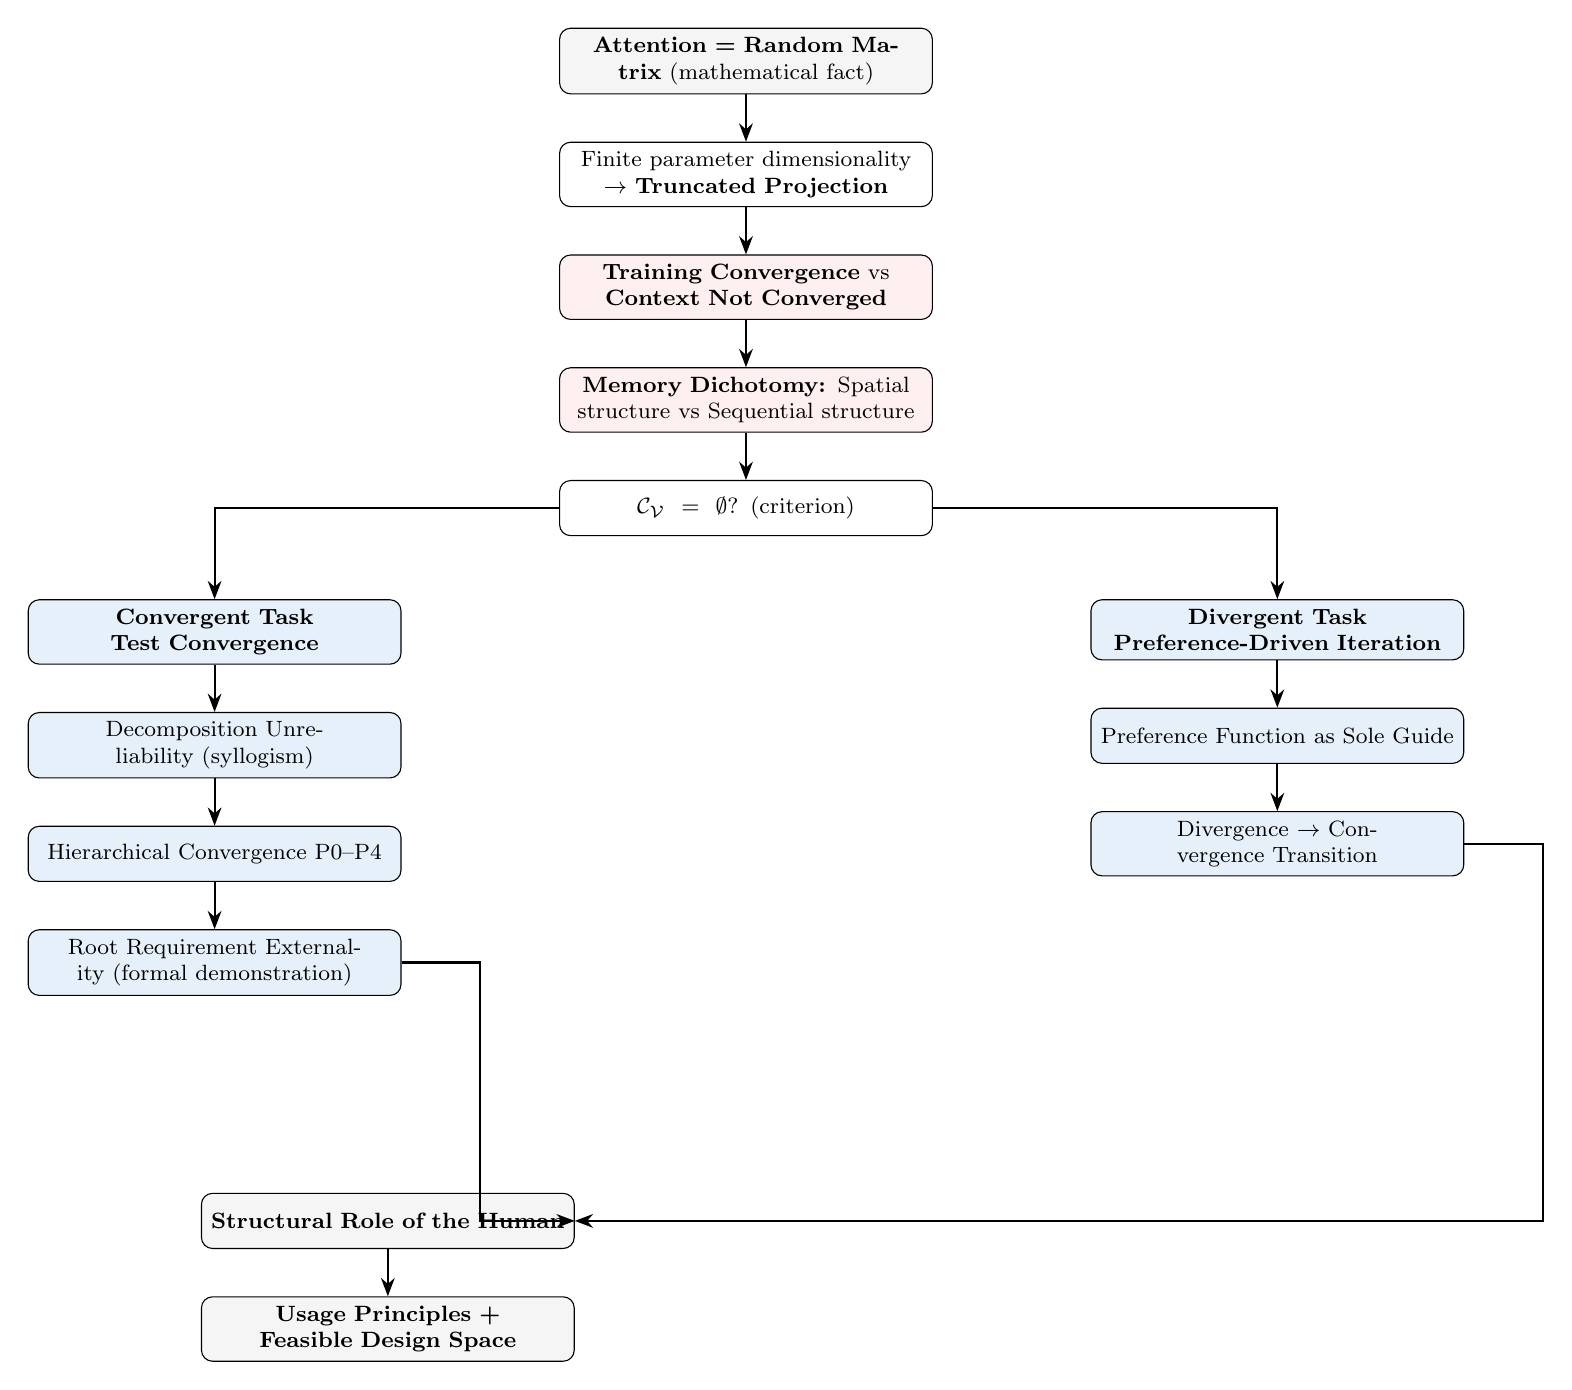
\begin{tikzpicture}[
    node distance=0.6cm,
    box/.style={rectangle,draw,rounded corners,text width=4.5cm,align=center,minimum height=0.7cm,font=\footnotesize},
    arrow/.style={-{Stealth},thick}
]
\node[box,fill=lightgray] (attn) {\textbf{Attention = Random Matrix} (mathematical fact)};
\node[box,below=of attn] (dim) {Finite parameter dimensionality $\to$ \textbf{Truncated Projection}};
\node[box,below=of dim,fill=lightred] (conv) {\textbf{Training Convergence} vs \textbf{Context Not Converged}};
\node[box,below=of conv,fill=lightred] (mem) {\textbf{Memory Dichotomy:} Spatial structure vs Sequential structure};
\node[box,below=of mem] (split) {$\verifspace = \emptyset$? (criterion)};

\node[box,fill=lightblue,below left=0.8cm and 2cm of split] (yes) {\textbf{Convergent Task}\\\textbf{Test Convergence}};
\node[box,fill=lightblue,below right=0.8cm and 2cm of split] (no) {\textbf{Divergent Task}\\\textbf{Preference-Driven Iteration}};

\node[box,fill=lightblue,below=of yes] (decomp) {Decomposition Unreliability (syllogism)};
\node[box,fill=lightblue,below=of decomp] (hier) {Hierarchical Convergence P0--P4};
\node[box,fill=lightblue,below=of hier] (root) {Root Requirement Externality (formal demonstration)};

\node[box,fill=lightblue,below=of no] (pref) {Preference Function as Sole Guide};
\node[box,fill=lightblue,below=of pref] (trans) {Divergence $\to$ Convergence Transition};

\node[box,fill=lightgray,below=2.5cm of root,xshift=2.2cm] (human) {\textbf{Structural Role of the Human}};
\node[box,fill=lightgray,below=of human] (eng) {\textbf{Usage Principles + Feasible Design Space}};

\draw[arrow] (attn) -- (dim);
\draw[arrow] (dim) -- (conv);
\draw[arrow] (conv) -- (mem);
\draw[arrow] (mem) -- (split);
\draw[arrow] (split) -| (yes);
\draw[arrow] (split) -| (no);
\draw[arrow] (yes) -- (decomp);
\draw[arrow] (decomp) -- (hier);
\draw[arrow] (hier) -- (root);
\draw[arrow] (no) -- (pref);
\draw[arrow] (pref) -- (trans);
\draw[arrow] (root.east) -- ++(1.0,0) |- (human);
\draw[arrow] (trans.east) -- ++(1.0,0) |- (human);
\draw[arrow] (human) -- (eng);
\end{tikzpicture}
\caption{Complete argument-chain diagram. Gray boxes = mathematical facts or synthetic conclusions; red boxes = core theoretical constructions; blue boxes = conceptual constructions. Arrows indicate logical dependency relations.}
\end{figure}

\section{Argument-Strength Tiering Standard}

\begin{table}[H]
\centering
\begin{tabular}{@{}p{2cm}p{5.5cm}p{5cm}@{}}
\toprule
\textbf{Tier} & \textbf{Criterion} & \textbf{Corresponding Content in This Paper} \\
\midrule
Rigorous tier & Mathematical fact, no approximation; ``$=$'' not ``$\approx$'' & \S\ref{sec:foundations}.1 (Attention = random matrix); \S\ref{sec:foundations}.4 (Operational convergence criteria) \\
Definitional tier & Formal stipulation of concepts, not involving truth-value judgments & \S\ref{sec:definitions}.1 (Core concept definition table) \\
Formal-demonstrative tier & Conclusions derived from explicit premises via valid inference steps, with both premises and inference rules publicly stated & \S\ref{sec:formal}.3--8 (Four derivations + syllogism + derivation of human role) \\
Conceptual-constructive tier & Core mechanism has attained conceptual precision, but overall derivation density has not yet reached the formal-demonstrative tier & \S\ref{sec:divergent_formal} (Divergent framework); \S\ref{sec:agi} (Convergent AGI argument) \\
Analogical tier & Conceptual correspondence holds but a known structural mismatch exists, honestly labeled in the text & \S\ref{sec:foundations}.7 (Multi-layer residual $\neq$ morphism composition) \\
Empirical-inferential tier & Observable predictions deduced from the theoretical framework, or empirical evidence cited from independent sources & \S\ref{sec:empirical} (Verification and predictions) \\
\bottomrule
\end{tabular}
\end{table}

\section{Placement of the Nine Framework Corollaries in This Paper}

\begin{table}[H]
\centering
\begin{tabular}{@{}c@{}p{8.5cm}@{}}
\toprule
\textbf{Corollary} & \textbf{Location in This Paper} \\
\midrule
1. Hallucination is structural necessity, not an engineering bug & \S\ref{sec:foundations}.5 (Truncated projection and convergence-coverage boundary); \S\ref{sec:definitions}.1 (Formal definition of out-of-distribution exposure risk) \\
2. Fine-tuning does not repair the unreliability of context & \S\ref{sec:open}.5 supplementary note (Memory dichotomy $\to$ fine-tuning does not touch the structural fact that context is not converged) \\
3. RAG does not create a new memory structure & \S\ref{sec:foundations}.6 (RAG manages context capacity); \S\ref{sec:open}.5 supplementary note \\
4. Task-domain阶梯 of verifiability density & \S\ref{sec:empirical}.1 table (Code $>$ Math $>$ Translation $>$ Open-ended writing) \\
5. Verification-signal mechanism of multi-agent debate & \S\ref{sec:empirical}.1 table and associated literature citations \\
6. Inverse-scaling expectation for overthinking & \S\ref{sec:empirical}.1; T5 (\S\ref{sec:empirical}.2) \\
7. The non-transitional nature of human intervention & \S\ref{sec:formal}.8 (Derivation of the structural role of the human) \\
8. Structural autonomy-reliability trade-off & C5 (\S\ref{sec:definitions}.2); T6 (\S\ref{sec:empirical}.2) \\
9. Plateau precedence in agent-task scaling & C6 (\S\ref{sec:definitions}.2); T1 (\S\ref{sec:empirical}.2); \S\ref{sec:open}.6 \\
\bottomrule
\end{tabular}
\end{table}

% ===================================================================
\newpage
\printbibliography

\end{document}
